% **************************************************************************************************************
% A Classic Thesis Style
% An Homage to The Elements of Typographic Style
%
% Copyright (C) 2015 André Miede http://www.miede.de
%
% If you like the style then I would appreciate a postcard. My address 
% can be found in the file ClassicThesis.pdf. A collection of the 
% postcards I received so far is available online at 
% http://postcards.miede.de
%
% License:
% This program is free software; you can redistribute it and/or modify
% it under the terms of the GNU General Public License as published by
% the Free Software Foundation; either version 2 of the License, or
% (at your option) any later version.
%
% This program is distributed in the hope that it will be useful,
% but WITHOUT ANY WARRANTY; without even the implied warranty of
% MERCHANTABILITY or FITNESS FOR A PARTICULAR PURPOSE.  See the
% GNU General Public License for more details.
%
% You should have received a copy of the GNU General Public License
% along with this program; see the file COPYING.  If not, write to
% the Free Software Foundation, Inc., 59 Temple Place - Suite 330,
% Boston, MA 02111-1307, USA.
%
% **************************************************************************************************************
\RequirePackage{fix-cm} % fix some latex issues see: http://texdoc.net/texmf-dist/doc/latex/base/fixltx2e.pdf
\documentclass[ twoside,openright,titlepage,numbers=noenddot,headinclude,%1headlines,% letterpaper a4paper
                footinclude=true,cleardoublepage=empty,abstractoff, % <--- obsolete, remove (todo)
                BCOR=5mm,paper=a4,fontsize=11pt,%11pt,a4paper,%
                ngerman,american,%
                ]{scrreprt}

%********************************************************************
% Note: Make all your adjustments in here
%*******************************************************
\input{classicthesis-config}

%********************************************************************
% Bibliographies
%*******************************************************
\addbibresource{Bibliography.bib}

%********************************************************************
% Hyphenation
%*******************************************************
%\hyphenation{put special hyphenation here}

% ********************************************************************
% GO!GO!GO! MOVE IT!
%*******************************************************
\begin{document}
\frenchspacing
\raggedbottom
\selectlanguage{spanish} % american ngerman
%\renewcommand*{\bibname}{new name}
%\setbibpreamble{}
\pagenumbering{roman}
\pagestyle{plain}
%********************************************************************
% Frontmatter
%*******************************************************
\include{FrontBackmatter/DirtyTitlepage}
\include{FrontBackmatter/Titlepage}
\thispagestyle{empty}

\hfill

\vfill

\noindent\myName: \textit{\myTitle,} \mySubtitle, \myDegree, 
\textcopyright\ \myTime

\bigskip

\noindent\spacedlowsmallcaps{Director}: \\
\myProf

\medskip

\noindent\spacedlowsmallcaps{Localización}: \\
\myLocation

\medskip

\noindent\spacedlowsmallcaps{Última modificación}: \\
\myTime

\cleardoublepage%*******************************************************
% Dedication
%*******************************************************
\thispagestyle{empty}
%\phantomsection 
\refstepcounter{dummy}
\pdfbookmark[1]{Dedicatoria}{Dedicatoria}

\vspace*{3cm}

\begin{center}
  A Cristina.
\end{center}
\cleardoublepage\include{FrontBackmatter/Foreword}
\cleardoublepage%*******************************************************
% Abstract
%*******************************************************
%\renewcommand{\abstractname}{Abstract}
\pdfbookmark[1]{Resumen}{Resumen}
\begingroup
\let\clearpage\relax
\let\cleardoublepage\relax
\let\cleardoublepage\relax

\myTodo[inline]{En el resumen/abstract debes ser menos negativo y dar algo más
  de detalle (aproximadamente doblar el tamaño del actual). Comenta cómo
  funciona el algoritmo implementado brevemente y no digas que la precisión no
  está cerca del estado del arte, sino que los resultados son coherentes a la
  descripción dada por los autores o algo así.}

\chapter*{Resumen}
En este trabajo se implementa un método para analizar dependencias
palabra a palabra con una estrategia de abajo a arriba
(\textit{Bottom-Up}) usando Máquinas de Soporte Vectoriales
(\textit{SVMs}). En concreto, este trabajo se ha centrado en analizar
las dependencias entre palabras en Castellano. Aunque la precisión de
los resultados no está cerca del estado del arte, es necesario tener
en cuenta que este parseador no usa información sobre la estructura de
las frases.

\paragraph{Etiquetas:} PNL, SVM, Parseo de dependencias.

\vfill

\begin{otherlanguage}{american}
  \pdfbookmark[1]{Abstract}{Abstract}
  \chapter*{Abstract}
  In this project, a method for analyzing word to word dependencies is
  implemented using a bottom-up strategy with the help of Support Vector
  machines. In particular, this work has focused in analyzing
  dependencies between words for spanish language. Even though accuracy
  is far from the state of the art, it is worth noting this parser is
  not using information about the sentences structure.
  \paragraph{Tags:} NLP, SVM, Dependency parsing.
\end{otherlanguage}

\endgroup			

\vfill
%\cleardoublepage\include{FrontBackmatter/Publications}
\cleardoublepage%*******************************************************
% Acknowledgments
%*******************************************************
\pdfbookmark[1]{Agradecimientos}{agradecimientos}

% \begin{flushright}{\slshape    
%     We have seen that computer programming is an art, \\ 
%     because it applies accumulated knowledge to the world, \\ 
%     because it requires skill and ingenuity, and especially \\
%     because it produces objects of beauty.} \\ \medskip
%     --- %\defcitealias{knuth:1974}{Donald E. Knuth}\citetalias{knuth:1974} \citep{knuth:1974}
% \end{flushright}

\begin{flushright}{\slshape
    An approximate answer to the right problem \\
    is worth a good deal more than an exact answer\\
    to an approximate problem.} \\ \medskip
    --- John Tukey
\end{flushright}

% \begin{flushright}{\slshape
%     People worry that computers will get too smart\\
%     and take over the world, but the real problem is\\
%     that they're too stupid and they've already taken\\
%     over the world.}  \\ \medskip
%     --- Pedro Domingos
% \end{flushright}  

\bigskip

\begingroup
\let\clearpage\relax
\let\cleardoublepage\relax
\let\cleardoublepage\relax
\chapter*{Agradecimientos}

Muchas gracias a mi familia por apoyarme durante todos estos años de carrera,
especialmente en los últimos meses de desarrollo de este proyecto. A mi tutor,
por apoyar la idea.

\bigskip

Y por último, a Cristina, por estar siempre ahí.

\endgroup




\pagestyle{scrheadings}
\cleardoublepage%*******************************************************
% Table of Contents
%*******************************************************
%\phantomsection
\refstepcounter{dummy}
\pdfbookmark[1]{\contentsname}{tableofcontents}
\setcounter{tocdepth}{2} % <-- 2 includes up to subsections in the ToC
\setcounter{secnumdepth}{3} % <-- 3 numbers up to subsubsections
\manualmark
\markboth{\spacedlowsmallcaps{\contentsname}}{\spacedlowsmallcaps{\contentsname}}
\tableofcontents 
\automark[section]{chapter}
\renewcommand{\chaptermark}[1]{\markboth{\spacedlowsmallcaps{#1}}{\spacedlowsmallcaps{#1}}}
\renewcommand{\sectionmark}[1]{\markright{\thesection\enspace\spacedlowsmallcaps{#1}}}
%*******************************************************
% List of Figures and of the Tables
%*******************************************************
\clearpage

\begingroup 
    \let\clearpage\relax
    \let\cleardoublepage\relax
    \let\cleardoublepage\relax
    %*******************************************************
    % List of Figures
    %*******************************************************    
    %\phantomsection 
    \refstepcounter{dummy}
    %\addcontentsline{toc}{chapter}{\listfigurename}
    \pdfbookmark[1]{\listfigurename}{lof}
    \listoffigures

    \vspace{8ex}

    %*******************************************************
    % List of TODOs
    % *******************************************************
    %\phantomsection 
    \refstepcounter{dummy}
    %\addcontentsline{toc}{chapter}{\listfigurename}
    \pdfbookmark[1]{Índice de TODOs}{lot}
    \listoftodos[TODO list]

    \vspace{8ex}
    
    %*******************************************************
    % List of Tables
    %*******************************************************
    %\phantomsection 
    \refstepcounter{dummy}
    %\addcontentsline{toc}{chapter}{\listtablename}
    \pdfbookmark[1]{\listtablename}{lot}
    \listoftables
        
    \vspace{8ex}
%   \newpage
    
    %*******************************************************
    % List of Listings
    %*******************************************************      
      %\phantomsection 
    \refstepcounter{dummy}
    %\addcontentsline{toc}{chapter}{\lstlistlistingname}
    \pdfbookmark[1]{\lstlistlistingname}{lol}
    \lstlistoflistings 

    \vspace{8ex}
       
    %*******************************************************
    % Acronyms
    %*******************************************************
    %\phantomsection 
    \refstepcounter{dummy}
    \pdfbookmark[1]{Acronyms}{acronyms}
    \markboth{\spacedlowsmallcaps{Acronyms}}{\spacedlowsmallcaps{Acronyms}}
    \chapter*{Acronyms}
    \begin{acronym}[SSyntSs]
        \acro{NLP}{Natural Language Processing}
        \acro{PNL}{Procesamiento del Lenguaje Natural}
        \acro{IA}{Inteligencia Artificial}
        \acro{QAS}{Question Answering Systems}
        \acro{SRA}{Sistemas de Respuesta a Preguntas}
        \acro{ASR}{Automatic Speech Recognition}
        \acro{RVA}{Reconocimiento de Voz Automático}
        \acro{UML}{Unified Modeling Language}
        \acro{POS}{Part-Of-Speech}
        \acro{AA}{Aprendizaje Automático}
        \acro{NER}{Named Entities}
        \acro{DP}{Dependency Parsing}
        \acro{HRL}{High-Resource Language}
        \acro{LRL}{Low-Resource Language}
        \acro{SDS}{Spoken Dialogue System}
        \acro{DM}{Dialogue Management}
        \acro{TTS}{Text-To-Speech}
        \acro{API}{Application Programming Interface}
        \acro{HTML}{Hyper Text Markup Language}
        \acro{CRF}{Conditional Random fields}
        \acro{PTB}{Penn Tree Bank}
        \acro{XML}{Extensible Markup Language}
        \acro{SO}{Semantic Orientation}
        \acro{PMI-IR}{Pointwise Mutual Information and Information Retrieval}
        \acro{SVM}{Support Vector Machine}
        \acro{SSyntSs}{Surface-Syntactic structures}
        \acro{DSyntSs}{Deep-Syntactic Structures}
        \acro{TDD}{Test-driven Development}
        \acro{BDD}{Behavior-Driven Development}
        \acro{FP}{Functional Programming}
    \end{acronym}                     
\endgroup

%********************************************************************
% Mainmatter
%*******************************************************
\cleardoublepage\pagenumbering{arabic}
%\setcounter{page}{90}
% use \cleardoublepage here to avoid problems with pdfbookmark
\cleardoublepage

\ctparttext{La memoria se organiza en cuatro partes.

  La primera, en el \autoref{ch:introduction}, es una introducción al
  Procesamiento del Lenguaje Natural, en ella se definen los tipos de
  aplicaciones que permite, así como una descripción del \emph{pipeline} usual
  que suele seguirse en este tipo de sistemas y el estado del arte.

  En la segunda parte, \autoref{ch:goals} se listan los objetivos del proyecto.

  La tercera parte se compone de los Capítulos~(\ref{ch:scalaintro}
  \ref{ch:algorithm} \ref{ch:impl} y \ref{ch:tdml}). En ellos se introduce al
  lenguaje \textsc{Scala}, se explican los detalles técnicos del algoritmo de
  parseo de dependencias, se discute la implementación y se muestran los casos
  de prueba realizados, respectivamente.

  Por último, la cuarta parte consta del \autoref{ch:eval} y
  \autoref{ch:future}, en donde se exponen los resultados obtenidos, se comparan
  los resultados con el algoritmo original y se proponen trabajos futuros.}

\part{Puesta en escena}
%************************************************
\chapter{Motivación e Introducción}\label{ch:introduction}
% ************************************************

\section{¿Qué es el Procesamiento del Lenguaje Natural?}
\label{sec:whatisnlp}

El lenguaje natural se refiere a cualquier lenguaje hablado por un humano, (\eg
Inglés, Castellano o Chino). El \ac{NLP}\marginpar{\acf{PNL}} es un campo de la
ciencia de la computación e ingeniería desarrollado a partir del estudio del
lenguaje y la computación lingüistica dentro del campo de la \ac{IA}. Los
objetivos del \ac{NLP} son diseñar y construir aplicaciones que faciliten la
interacción humana con la máquinas y otros dispositivos mediante el uso del
lenguaje natural. Dentro del amplio campo del \ac{NLP} podemos distinguir las
siguientes áreas principales:

\begin{description}\label{sec:nlpfields}
  \item[QAS:] \ac{QAS}\marginpar{\acf{SRA}}. En estos sistemas se pretende
    remplazar a los usuales buscadores en los que introducimos un texto para
    obtener algún tipo de respuesta a una pregunta. Por ejemplo, si quisieramos
    saber a qué hora abre un centro comercial, bastaría con hablarle al sistema
    en lenguaje natural -- nuestro lenguaje natural, ya sea Inglés, Alemán o
    Castellano y el sistema nos daría respuesta a nuestra pregunta. Aunque ya
    existen este tipo de sistemas (\eg \emph{Siri, Cortana\dots}) están aún en
    una situación muy precaria, ya que ninguno entiende por completo el lenguaje
    natural, solo un subconjunto de frases clave.
  \item[Resúmenes:] Este área incluye aplicaciones que puedan, basándose en una
    colección de documentos, dar como salida un resumen coherente del contenido
    de los mismos. Otra de las posibles aplicaciones sería generar
    presentaciones a partir de dichos documentos.
  \item[Traducción:] Esta fue la principal área de investigación en el campo del
    \ac{NLP}. Como claro ejemplo tenemos el traductor de Google, mejorando día a
    día. Sin embargo, un traductor realmente útil sería aquel que consiga
    traducir en tiempo real una frase que le dictemos mientras decidimos qué
    línea de autobús debemos coger para llegar a tiempo a una conferencia en
    Zurich.
  \item[Reconocimiento de voz:] Una de las tareas más difíciles en \ac{NLP}. Aún
    así, se han conseguido grandes avances en la construcción de modelos que
    pueden usarse en el teléfono móvil o en el ordenador. Estos modelos son
    capaces de reconocer expresiones del lenguaje hablado como preguntas y
    comandos. Desafortunadamente, los sistemas \ac{ASR}\marginpar{\acf{RVA}}
    funcionan bajo dominios muy acotados y no permiten al interlocutor desviarse
    de la entrada que espera el sistema, \eg \emph{``Por favor, diga ahora la
      opción a elegir: 1 Para\dots, 2 para\dots''}
  \item[Clasificación de documentos:] Una de las áreas más exitosas del
    \ac{NLP}, cuyo objetivo es identificar a qué categoría debería pertenecer un
    documento. Ha demostrado tener un amplio abanico de aplicaciones, \eg
    filtrado de \emph{spam}, clasificación de artículos de noticias,
    valoraciones de películas\dots Parte de su éxito e impacto se debe a la
    facilidad relativa que conlleva entrenar los modelos de aprendizaje para
    hacer dichas clasificaciones.
\end{description}

El \ac{NLP} emplea técnicas computacionales con el propósito de aprender,
entender y producir lenguaje humano. Las aproximaciones de hace unos años en el
campo de la investigación del lenguaje se centraban en automatizar el análisis
de las estructuras lingüísticas y desarrollar tecnologías como las mencionadas
anteriormente. Los investigadores de hoy en día se centran en usar dichas
herramientas en aplicaciones para el mundo real, creando sistemas de diálogo
hablados y motores de traducción \emph{Speech-to-Speech}, es decir, dados dos
interlocutores, interpretar y traducir sus frases. Otro de los focos en los que
se centran las investigaciones actuales son la minería en redes sociales en
busca de información sobre salud, finanzas e identificar los sentimietos y
emociones sobre determinados productos. 

\section{Historia del Procesamiento del Lenguaje Natural}
\label{sec:currentnlp}

A continuación, citamos algunos de los avances en este campo durante los últimos
años según \citet{Hirschberg2015}.

Durante las primeras épocas de esta ciencia, se intentaron escribir vocabularios
y reglas del lenguaje humano para que el ordenador las entendiera. Sin embargo,
debido a la naturaleza ambigua, variable e interpretación dependiente del
contexto de nuestro lenguaje resultó una ardua tarea. Por ejemplo, una estrella
puede ser un ente astronómico o una persona, y puede ser un nombre o un verbo.

En la década de los 90, los investigadores transformaron el mundo del \ac{NLP}
desarrollando modelos sobre grandes cantidades de datos sobre lenguajes. Estas
bases de datos se conocen como \emph{corpus}. El uso de estos conjuntos de datos
fueron uno de los primeros éxitos notables del uso del \emph{big data}, mucho
antes de que el \ac{AA} acuñara este término.

Esta aproximación estadística al \ac{NLP} descubrió que el uso de métodos
simples usando palabras, secuencias del \emph{\ac{POS}}\marginpar{\ac{POS}: Categorías
  morfosintácticas en castellano} (si una palabra es un nombre, verbo o
preposición), o plantillas simples pueden obtener buenos resultados cuando son
entrenados sobre un gran conjunto de datos. A día de hoy, muchos sistemas de
clasificación de texto y sentimientos se basan únicamente en los distintos
conjuntos de palabras o \emph{``bag of words''} que contienen los documentos,
sin prestar atención a su estructura o significado. El estado del arte de hoy
día usa aproximaciones con \ac{AA} y un rico conocimiento de la estructura
lingüística. Un ejemplo de estos sistemas es \emph{Stanford CoreNLP}
\citep{Manning2014}. \emph{CoreNLP} proporciona un \emph{pipeline} estándar para
el procesamiento del \ac{NLP} incluyendo:

\begin{description}
  \item[POS Tagging:] o etiquetado morfosintáctico. Módulo encargado de leer
    texto en algún lenguaje y asignar la categoría morfosintáctica a cada
    palabra, \eg nombre, verbo, adjetivo\dots aunque por lo general se suelen
    usar etiquetas más detalladas como ``\emph{nombre-plural}''.
  \item[NER:] \ac{NER}, etiqueta palabras en un texto correspondientes a
    \emph{nombres de cosas}, como personas, nombres de compañías, nombres de
    proteínas o genes etc. En concreto, \emph{CoreNLP} distingue de forma muy
    precisa tres tipos de clases, personas, organizaciones y localizaciones.
  \item[Parseo Gramatical:] Resuelve la estructura gramatical de frases, \eg qué
    grupos de palabras van juntos formando frases y qué palabras son sujeto u
    objeto de un verbo. Como se ha comentado, en aproximaciones anteriores se
    usaban parseadores probabilísticos usando conocimiento del lenguaje a partir
    de sentencias analizadas sintácticamente a mano. Para así producir el
    análisis más probable de sentencias nuevas. Actualmente se se usan
    parseadores estadísticos, los cuales aún comenten fallos, pero funcionan
    bien a rasgos generales.
  \item[DP:] \ac{DP} o parseo de dependencias. Analiza la estructura gramatical
    de una frase, estableciendo relaciones entre palabras principales y palabras
    que modifican dichas palabras principales. La \autoref{fig:nndep} muestra un
    ejemplo. La flecha dirigida de la palabra \emph{moving} a la palabra
    \emph{faster} indica que \emph{faster} modifica a \emph{moving}. La flecha
    está etiquetada con una palabra, en este caso \emph{advmod}, indicando la
    naturaleza de esta dependencia. La \autoref{fig:corenlp} muestra ejemplos de
    los distintos módulos del \emph{pipeline} de \emph{CoreNLP}
\end{description}

\begin{figure}[bth]
  \includegraphics[width=1\linewidth]{gfx/nndep-example}
  \caption[Ejemplo de parseo de dependencias]{Ejemplo de parseo de dependencias}
  \label{fig:nndep}
\end{figure}

\begin{figure}[bth]
  \makebox[\textwidth][c]{\includegraphics[width=1.5\textwidth]{gfx/corenlp}}
  \caption[Ejemplo de parseo de dependencias]{Many language technology tools start by doing linguistic structure analysis. Here we show output from Stanford CoreNLP. As shown from top to
bottom, this tool determines the parts of speech of each word, tags various words or phrases as semantic named entities of various sorts, determines which entity
mentions co-refer to the same person or organization, and then works out the syntactic structure of each sentence, using a dependency grammar analysis.}
  \label{fig:corenlp}
\end{figure}

\section{Limitaciones}
\label{sec:nlplimits}

Aunque se han producido avances, una de las principales limitaciones del
\ac{NLP} hoy día es el hecho de que la mayoría de recursos y sistemas solo están
disponibles para los denominados \acp{HRL}\marginpar{\ac{HRL}: Idiomas de altos
recursos}, estos lenguajes son el Inglés, Francés, Español, Alemán y Chino. Por
contra, hay una gran cantidad de \acp{LRL} --\marginpar{\ac{LRL}: Idiomas de bajos
recursos} como Bengalí, Indonesio, Punjabí, Cebuano y Swahili -- hablados y
escritos por millones de personas que no disponen de este tipo de sistemas. Uno
de los mayores retos para la comunidad del lenguaje es desarrollar recursos y
herramientas para cientos o miles de lenguajes, no solo para unos pocos.



\cleardoublepage
\part{Objetivos}
%*****************************************
\chapter{Parseo de dependencias en Español}\label{ch:depparsing}
% *****************************************

\todo[inline]{Desribir de forma más detallada el Dep Parsing, mencionar state of
  the art (3/4 papers), entre ellos el implementado}

\todo[inline]{Sección con algoritmo implementado, reiterando sección anterior
  pero con lujo de detalles (Teóricos y código)}

% Los titulas como te digo y extiendes un poco lo que se hace en cada uno de ellos
% (3-4 frases por objetivo):

% - Revisión bibliográfica del estado del arte y antecedentes del dep parsing en
% español. (Enlazas con capitulos de la memoria de antecedentes y dep parsing)

% - Elección y análisis de requerimientos de un procedimiento apropiado de dep
% parsing a partir de la revisión anterior y diseño del mismo para el lenguaje de
% programación Scala (Enlazas con la explicación teórica del algoritmo que has
% implementado y con un capítulo de introducción a Scala).

% - Implementación y procesos de prueba del algoritmo escogido. (Capítulos de
% implementación del algoritmo y de tests de ingeniería del software)

% - Evaluación del algoritmo, comparación y discusión de resultados obtenidos en
% casos prácticos (Capítulo sobre resultados obtenidos, comparación con los
% resultados originales y otros disponibles y último capítulo de conclusiones).

% Los objetivos mencionan la resolución del trabajo como uno de ellos, pero sin
% entrar en detalle tal y como en el que se entra en los capítulos
% correspondientes. La sección de objetivos se limita a enumerarlos y explicar
% brevemente en qué consisten. En la Resolución del trabajo, te explicas con todo
% lujo de detalles técnicos y científicos sobre los métodos desarrollados.

A continuación se listan los objetivos previstos del trabajo.

\paragraph{Revisión bibliográfica del estado del arte y antecedentes del parseo
  de dependencias en Español.} Este objetivo pretende explorar los métodos
existentes que realizan parseado de dependencias, para adquirir un conocimiento
previo del \nameref{sec:stateoftheart} en la literatura. Así como conocer los
métodos existentes para el parseo de dependencias en Español
\cite{ballesteros2016}.

\paragraph{Elección y análisis de requerimientos de un procedimiento apropiado de
  parseo de dependencias y diseño para Scala}
Debido a la popularidad del lenguaje de programación \textsc{Scala} en el área
del \ac{AA} y la minería de datos, se pretende implementar este trabajo bajo
dicho lenguaje.\myTodo{Enlazar con explicación algoritmo implementado, y
  capítulo de intro a \textsc{scala}}. El algoritmo de parseo de dependencias
elegido se ha basado en \citeauthor{yamada2003} \cite{yamada2003} y
\citeauthor{rohit2016} \cite{rohit2016}.

\paragraph{Implementación y procesos de prueba del algoritmo escogido}



\paragraph{Evaluación del algoritmo, comparación y discusión de resultados
  obtenidos en casos prácticos}


%*****************************************
%*****************************************
%*****************************************
%*****************************************
%*****************************************

%\addtocontents{toc}{\protect\clearpage} % <--- just debug stuff, ignore
\ctparttext{Esta parte del trabajo se centra en los pasos seguidos para el
  desarrollo del proyecto. Se organiza como sigue:
  
  En el \autoref{ch:scalaintro} se discuten las características del lenguaje
  \textsc{Scala}, y por qué ha sido escogido para el desarrollo.

  El \autoref{ch:algorithm} detalla los aspéctos técnicos del algoritmo de
  parseo de dependencias seleccionado.

  En el \autoref{ch:impl} se narra las distintas etapas seguidas para el
  desarrollo, desde el análisis hasta la implementación.

  Por último, el \autoref{ch:tdml} explica los distintos casos de prueba
  llevados a cabo.
}
\part{Resolución del Trabajo}
%************************************************
\chapter{Una Introducción a Scala}
\label{ch:scalaintro}
%************************************************

El nombre \textsc{Scala} es una concatenación de dos palabras, \emph{Scalable
  Language}. A continuación se enumeran algunas de las razonas por las que se ha
elegido este lenguaje, la lista completa puede encontrarse en
\citeauthor{Dean2015} \cite{Dean2015}.

\section{¿Por qué \textsc{Scala}?}
\label{sec:whyscala}

Las principales características de \textsc{Scala} que lo hacen un buen candidato
para este trabajo son las siguientes:

\begin{description}
\item[Paradigma mixto --- Programación Orientada a Objetos:] \textsc{Scala}
  soporta al completo el paradigma de la orientación a objetos. Además, mejora
  el modelo de objetos proporcionado por \textsc{Java} con la introducción de
  \textsc{Traits}, un modo muy claro de implementar tipos mediante composiciones
  mixtas. Todo es un objeto en \textsc{Scala}, incluso los tipos numéricos.
\item [Paradigma mixto --- Programación Funcional:] De igual modo, \textsc{Scala}
  soporta al completo \acfi{FP}\acused{FP}\graffito{\ac{FP}: Programación
    Funcional}. En los últimos años, la \ac{FP} ha resurgido como una de las
  mejores herramientas para pensar en problemas de concurrencia, \emph{Big Data}
  y en general para escribir código \enhancement{correctness}correcto. Este
  código correcto, conciso y potente se logra mediante el uso de valores
  inmutables, funciones de primera clase, funciones sin efectos colaterales,
  funciones de ``orden superior'' y colecciones de funciones.
\item [Sintaxsis breve, elegante y flexible:] Expresiones que pueden llegar a
  ser demasiado extensas en \textsc{Java} se hacen concisas en \textsc{Scala}.
\item [Arquitectura Scalable:] \textsc{Scala} permite escribir desde
  \emph{scripts} pequeños, que son interpretados, hasta aplicaciones
  distribuidas de gran envergadura. Hay cuatro mecanismos inherentes al lenguaje
  permitiendo esta escalabilidad: 1) composiciones mixtas mediante
  \textsc{Traits}, 2) miembros de tipo abstracto y genéricos; 3) anidamiento de
  clases y 4) tipos explícitos \textsc{self}.
  
\end{description}

%*****************************************
%*****************************************
%*****************************************
%*****************************************
%*****************************************

%************************************************
\chapter{Elección del Algoritmo}
\label{ch:algorithm}
%************************************************
\citeauthor{yamada2003} \cite{yamada2003} proponen un método para analizar las
dependencias palabra-a-palabra mediante una estrategia \emph{bottom-up} -- de
abajo a arriba. -- Para ello se hace uso de la técnica de \ac{AA}
\acfi{SVM}. Sus experimentos se basan en árboles de dependencias creados a
partir del corpus \ac{PTB}, logrando una precisión superior al 90\% para
dependencias palabra-a-palabra. Aún siendo esta precisión inferior al
\nameref{sec:stateoftheart}, hay que tener en cuenta que este método no utiliza
información sobre la estructura de las frases.

El tipo de anotaciones usadas en este método pueden verse en la
\autoref{fig:deptree}. Esta forma de ilustrar las dependencias palabra-a-palabra
es más sencilla de entender para los anotadores que el usual estilo \ac{PTB} ---
\autoref{fig:strtree} --- Además, la representación del árbol de dependencias de
la \autoref{fig:deptree} hace que la construcción de los datos de entrenamiento
sea menos ruidosa, al ser el proceso de anotación más simple.

\begin{figure}[h]
%\resizebox{1.3\textwidth}{!}{%
\tiny
\begin{tikzpicture}[every node/.style={align=center}]
  \tikzset{
    edge from parent/.style={
      draw,edge from parent
      path={(\tikzparentnode.south)-- +(0,-8pt)-| (\tikzchildnode)}
    },
    frontier/.style={distance from root=208pt}, % Align leaf nodes
    level 1+/.style={level distance=18pt} % Distance between levels
  }

   \Tree [.S
             [.NP Rolls-Royce\\NNP Motor\\NNP Cars\\NNPS Inc\\NNP ]
             [.VP said\\VBD
                [.SBAR [.none ]
                   [.S
                      [.NP it\\PRP ]
                      [. VP expects\\VBZ
                         [.S
                            [.NP its\\PRP\$ U.S\\NNP sales\\NNS ]
                            [.VP to\\TO
                               [.VP remain\\VB
                                  [.ADJP steady\\JJ ]
                                  [.PP at\\IN
                                     [.NP
                                        [.QP about\\IN 1200\\CD ]
                                        cars\\NNS
                                     ]
                                  ]
                               ]
                            ]
                         ]
                      ]
                   ]
                ]
             ]
         ]
\end{tikzpicture}
%}
\caption{Estructura en árbol de la frase ``Rolls-Royce Motor Cars Inc. said it
  expects its U.S. sales to remain steady at about 1,200 cars.''}
\label{fig:strtree}
\end{figure}

\begin{figure}[th]
  \scriptsize
  \begin{tikzpicture}[every node/.style={align=center},level distance=30pt]
    \tikzset{edge from parent/.append style={<-, >=latex,thick}}
   \Tree [.said\\VBD 
             [.Inc.\\NNP Rolls-Royce\\NNP Motor\\NNP Cars\\NNPS ]
             [.expects\\VBZ it\\PRP
                [.remain\\VB
                   [.sales\\NNS its\\PRP\$ U.S\\NNP ]
                   to\\TO
                   steady\\JJ 
                   [.at\\IN [.cars\\NNS [.about\\IN 1200\\CD ] ] ]
                ]
             ]
           ]
   \end{tikzpicture}
   \caption{Árbol de parseo de dependencias}
   \label{fig:deptree}
\end{figure}


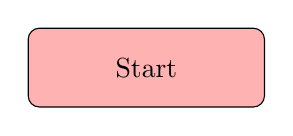
\begin{tikzpicture}[node distance=2cm]
\tikzstyle{startstop} = [rectangle, rounded corners, minimum width=3cm, minimum height=1cm,text centered, draw=black, fill=red!30]
\node (start) [startstop] {Start};

\end{tikzpicture}

 
%*****************************************
%*****************************************
%*****************************************
%*****************************************
%*****************************************

%************************************************
\chapter{Implementación}
\label{ch:impl}
%************************************************

%*****************************************
%*****************************************
%*****************************************
%*****************************************
%*****************************************

%************************************************
\chapter{Casos de Prueba}
\label{ch:tests}
%************************************************
\myTodo[inline]{Hay que escribir los Tests aún}
%*****************************************
%*****************************************
%*****************************************
%*****************************************
%*****************************************

\ctparttext{Esta última parte de la memoria se dedica a presentar los resultados
  obtenidos con el parseador introducido en \autoref{ch:algorithm}, así como
  comparar los resultados con la implementación original. Por último, se
  comentarán algunas ideas para trabajos futuros.  }
\part{Conclusiones y vías futuras}
%************************************************
\chapter{Evaluación, Comparación y Discusión de Resultados}
\label{ch:eval}
%************************************************

\section{Método de Evaluación}
\label{sec:eval}

\section{Resultados}
\label{sec:results}

\section{Comparación de Resultados}
\label{sec:compresult}

\section{Trabajo Futuro}
\label{sec:future}

%*****************************************
%*****************************************
%*****************************************
%*****************************************
%*****************************************

%************************************************
\chapter{Vías Futuras}
\label{ch:future}
%************************************************

\section{Trabajo Futuro}
\label{sec:future}

Como trabajo futuro se podrían implementar distintos tipos de algoritmos y
establecer una comparación entre ellos.

Otra posible mejora puede ser aprovechar aún más las características de
\textsc{Scala}, ya que al momento de escribir el programa, el desarrollador se
estaba familiarizando con el lenguaje. Hay mucho margen para realizar mejoras en
el código. Por ejemplo, se podría hacer todo el código funcional e
inmutable.

\myTodo[inline]{El trabajo futuro debe ir en el capítulo de
  conclusiones y contener al menos 3 puntos. Uno de ellos es obvio,
  implementar más algoritmos. También construir más procesos de
  pipeline. Otro sería irse a Big Data, algoritmos implementados en
  Spark por ejemplo. }

%*****************************************
%*****************************************
%*****************************************
%*****************************************
%*****************************************

%\include{multiToC} % <--- just debug stuff, ignore for your documents
% ********************************************************************
% Backmatter
%*******************************************************
\appendix
%\renewcommand{\thechapter}{\alph{chapter}}
\cleardoublepage
\part{Apéndice}
%\include{Chapters/Chapter0A}
%********************************************************************
% Other Stuff in the Back
%*******************************************************
\cleardoublepage\include{FrontBackmatter/Bibliography}
\cleardoublepage%*******************************************************
% Declaration
%*******************************************************
\refstepcounter{dummy}
\pdfbookmark[0]{Declaración}{declaracion}
\chapter*{Declaración}
\thispagestyle{empty}

Yo, \textsc{Alejandro Alcalde Barros}, alumno del \textsc{Grado en Ingeniería
Informática} de la \textsc{Escuela Técnica Superior de Ingenierías Informática y
de Telecomunicaciones} de la \textsc{Universidad de Granada}, declaro
explícitamente que el trabajo presentado es original, entendiéndose en el
sentido de que no se ha utilizado ninguna fuente sin citarla debidamente.

\bigskip
 
\noindent\textit{\myLocation, \myTime}

\smallskip

\begin{flushright}
    \begin{tabular}{m{5cm}}
        \\ \hline
        \centering\myName \\
    \end{tabular}
\end{flushright}

\cleardoublepage\include{FrontBackmatter/Colophon}
% ********************************************************************
% Game Over: Restore, Restart, or Quit?
%*******************************************************
\end{document}
% ********************************************************************
